\documentclass[11pt,a4paper]{article}
\usepackage[a4paper,margin=0.72in]{geometry}
\usepackage{amsmath,amssymb,mathtools}
\usepackage{microtype}
\usepackage{lmodern}
\usepackage[T1]{fontenc}
\usepackage{enumitem}
\usepackage{booktabs,array}
\usepackage{xcolor}
\usepackage{tikz}
\usepackage{pgfplots}
\pgfplotsset{compat=1.18}
\usetikzlibrary{arrows.meta,calc,patterns,positioning,decorations.pathmorphing,shadings}
\usepackage[most]{tcolorbox}
\usepackage{hyperref}
\hypersetup{colorlinks=true,linkcolor=blue!50!black,urlcolor=blue!50!black}
\usepackage{float}
\usepackage{caption}
\usepackage{placeins}

\definecolor{ink}{HTML}{122033}
\definecolor{accent}{HTML}{2F6690}
\definecolor{soft}{HTML}{F3F7FA}
\definecolor{softtwo}{HTML}{EEF6F0}
\definecolor{warn}{HTML}{FFF5E6}
\definecolor{lineblue}{HTML}{1D4E89}
\definecolor{linegreen}{HTML}{2E7D32}
\definecolor{lineorange}{HTML}{D97706}
\definecolor{linepurple}{HTML}{6D28D9}

\setlength{\parindent}{0pt}
\setlength{\parskip}{0.45em}
\setlist[itemize]{topsep=0.3em,itemsep=0.2em,leftmargin=1.4em}
\setlist[enumerate]{topsep=0.3em,itemsep=0.3em,leftmargin=1.6em}

\newtcolorbox{methodbox}{enhanced,breakable,colback=soft,colframe=accent!75!black,boxrule=0.7pt,arc=2mm,left=1.5mm,right=1.5mm,top=1mm,bottom=1mm,title=Method / reasoning plan,fonttitle=\bfseries}
\newtcolorbox{answerbox}{enhanced,breakable,colback=softtwo,colframe=linegreen!70!black,boxrule=0.7pt,arc=2mm,left=1.5mm,right=1.5mm,top=1mm,bottom=1mm,title=Final answer,fonttitle=\bfseries}
\newtcolorbox{notebox}{enhanced,breakable,colback=warn,colframe=lineorange!80!black,boxrule=0.7pt,arc=2mm,left=1.5mm,right=1.5mm,top=1mm,bottom=1mm,title=Source/interpretation note,fonttitle=\bfseries}
\newcommand{\R}{\mathbb{R}}
\newcommand{\dd}{\,d}
\newcommand{\grad}{\nabla}
\newcommand{\norm}[1]{\left\lVert #1\right\rVert}
\newcommand{\pd}[2]{\frac{\partial #1}{\partial #2}}
\newcommand{\abs}[1]{\left\lvert #1\right\rvert}

\title{\textbf{Multivariable Calculus: Problem Set 8}\\Detailed Assignment-Style Solutions with Diagrams}
\author{Prepared solution set}
\date{}

\begin{document}
\maketitle
\tableofcontents
\newpage

\section*{Conventions used throughout}
\addcontentsline{toc}{section}{Conventions used throughout}
The goal of these solutions is to show the full calculation path, not only the final answer.  For every optimization problem, I first identify the feasible set, reduce the number of variables whenever possible, and then check whether maxima/minima exist from compactness or from an unbounded direction.  For every integral problem, I first write the region or solid explicitly, because a wrong region almost always gives a wrong integral.

\begin{methodbox}
For constrained extrema with one or two constraints, I use one of two methods.
\begin{enumerate}[label=\arabic*.]
\item If the constraints allow direct substitution, I reduce to fewer variables and optimize the reduced expression.
\item If direct substitution is less convenient, I use Lagrange multipliers: at an interior constrained extremum, the gradient of the objective lies in the span of the gradients of the active constraints.
\end{enumerate}
For integrals, I always write the region in inequalities before integrating.  This is the main check that prevents accidental reversal of limits.
\end{methodbox}

\section{Problem 1: Extreme values with two constraints}

\subsection{Problem 1(i)}
Find the extreme values of
\[
 f(x,y,z)=x+2y
\]
subject to
\[
 x+y+z=1,\qquad y^2+z^2=4.
\]

\begin{methodbox}
The first constraint is a plane and the second constraint is a circular cylinder in the \(yz\)-variables.  The plane lets us solve for \(x\).  Then the objective becomes a linear function on the circle \(y^2+z^2=4\).  A linear function on a circle is maximized in the direction of its coefficient vector and minimized in the opposite direction.
\end{methodbox}

From the plane,
\[
 x=1-y-z.
\]
Substitute this into \(f\):
\[
 f=x+2y=(1-y-z)+2y=1+y-z.
\]
Thus we need to maximize and minimize
\[
 1+y-z
\]
subject to
\[
 y^2+z^2=4.
\]
The variable part is
\[
 y-z=(1,-1)\cdot (y,z).
\]
The vector \((1,-1)\) has length
\[
 \sqrt{1^2+(-1)^2}=\sqrt2.
\]
On the circle of radius \(2\), the largest possible value of \((1,-1)\cdot(y,z)\) is
\[
 2\sqrt2,
\]
and the smallest possible value is
\[
 -2\sqrt2.
\]
Therefore,
\[
 f_{\max}=1+2\sqrt2,\qquad f_{\min}=1-2\sqrt2.
\]

The maximum occurs when \((y,z)\) points in the direction \((1,-1)\):
\[
 (y,z)=2\frac{(1,-1)}{\sqrt2}=(\sqrt2,-\sqrt2).
\]
Then
\[
 x=1-y-z=1-\sqrt2+\sqrt2=1.
\]
The minimum occurs at the opposite point:
\[
 (y,z)=(-\sqrt2,\sqrt2),\qquad x=1.
\]

\begin{figure}[H]
\centering
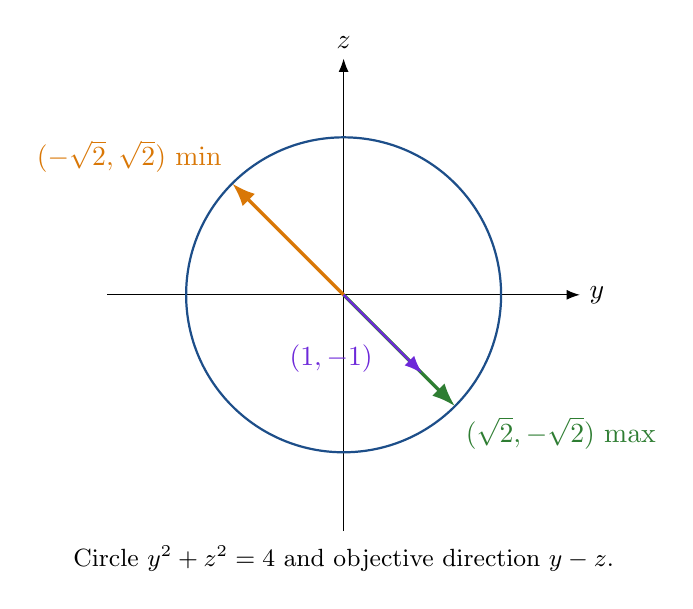
\begin{tikzpicture}[scale=1.0,>=Latex]
\draw[->] (-3,0)--(3,0) node[right]{$y$};
\draw[->] (0,-3)--(0,3) node[above]{$z$};
\draw[lineblue,thick] (0,0) circle (2);
\draw[->,linegreen,very thick] (0,0)--(1.414,-1.414) node[below right]{$(\sqrt2,-\sqrt2)$ max};
\draw[->,lineorange,very thick] (0,0)--(-1.414,1.414) node[above left]{$(-\sqrt2,\sqrt2)$ min};
\draw[->,linepurple,thick] (0,0)--(1,-1) node[midway,below left]{$(1,-1)$};
\node at (0,-3.35){\small Circle $y^2+z^2=4$ and objective direction $y-z$.};
\end{tikzpicture}
\caption{Reduction of Problem 1(i) to a linear objective on a circle in the \((y,z)\)-plane.}
\end{figure}

\begin{answerbox}
\[
\boxed{f_{\max}=1+2\sqrt2\text{ at }(1,\sqrt2,-\sqrt2)}
\]
\[
\boxed{f_{\min}=1-2\sqrt2\text{ at }(1,-\sqrt2,\sqrt2)}
\]
\end{answerbox}

\subsection{Problem 1(ii)}
Find the extreme values of
\[
 f(x,y,z)=3x-y-3z
\]
subject to
\[
 x+y-z=0,\qquad x^2+2z^2=1.
\]

The plane gives
\[
 y=z-x.
\]
Substitute into \(f\):
\[
 f=3x-(z-x)-3z=4x-4z=4(x-z).
\]
Thus the problem reduces to maximizing/minimizing
\[
 4x-4z
\]
subject to
\[
 x^2+2z^2=1.
\]

Write this as an ellipse.  We optimize the linear form
\[
 a\cdot (x,z),\qquad a=(4,-4),
\]
under the quadratic constraint
\[
 (x,z)^TQ(x,z)=1,
\qquad Q=\begin{pmatrix}1&0\\0&2\end{pmatrix}.
\]
For an ellipse of the form \(u^TQu=1\), the maximum value of \(a\cdot u\) is
\[
 \sqrt{a^TQ^{-1}a}.
\]
Here
\[
 Q^{-1}=\begin{pmatrix}1&0\\0&1/2\end{pmatrix},
\]
so
\[
 a^TQ^{-1}a=4^2+(-4)^2\frac12=16+8=24.
\]
Therefore
\[
 f_{\max}=\sqrt{24}=2\sqrt6,
\qquad f_{\min}=-2\sqrt6.
\]
The maximizing point in \((x,z)\) is
\[
 (x,z)=\frac{Q^{-1}a}{\sqrt{a^TQ^{-1}a} }
 =\frac{(4,-2)}{2\sqrt6}
 =\left(\frac{2}{\sqrt6},-\frac{1}{\sqrt6}\right).
\]
Then
\[
 y=z-x=-\frac{1}{\sqrt6}-\frac{2}{\sqrt6}=-\frac{3}{\sqrt6}=-\frac{\sqrt6}{2}.
\]
The minimizing point is the negative of this point in the \((x,z)\)-ellipse:
\[
 (x,z)=\left(-\frac{2}{\sqrt6},\frac{1}{\sqrt6}\right),
\qquad y=\frac{\sqrt6}{2}.
\]

\begin{answerbox}
\[
\boxed{f_{\max}=2\sqrt6\text{ at }\left(\frac{2}{\sqrt6},-\frac{\sqrt6}{2},-\frac{1}{\sqrt6}\right)}
\]
\[
\boxed{f_{\min}=-2\sqrt6\text{ at }\left(-\frac{2}{\sqrt6},\frac{\sqrt6}{2},\frac{1}{\sqrt6}\right)}
\]
\end{answerbox}

\subsection{Problem 1(iii)}
Find the extreme values of
\[
 f(x,y,z)=yz+xy
\]
subject to
\[
 xy=1,
\qquad y^2+z^2=1.
\]

The constraint \(xy=1\) gives
\[
 x=\frac1y,
\]
so \(y\neq0\).  Then
\[
 f=yz+xy=yz+1.
\]
Thus the problem is equivalent to maximizing/minimizing \(yz+1\) on the circle
\[
 y^2+z^2=1.
\]
For real numbers \(y,z\),
\[
 (y-z)^2\ge0
\]
implies
\[
 y^2+z^2-2yz\ge0.
\]
Since \(y^2+z^2=1\), we get
\[
 yz\le \frac12.
\]
Similarly,
\[
 (y+z)^2\ge0
\]
implies
\[
 y^2+z^2+2yz\ge0,
\]
so
\[
 yz\ge -\frac12.
\]
Therefore
\[
 \frac12\le yz+1\le \frac32.
\]
The maximum \(yz=1/2\) occurs when \(y=z=1/\sqrt2\) or \(y=z=-1/\sqrt2\).  The minimum \(yz=-1/2\) occurs when \(z=-y\) and \(|y|=1/\sqrt2\).

\begin{answerbox}
\[
\boxed{f_{\max}=\frac32}
\]
attained at
\[
\boxed{(x,y,z)=\left(\sqrt2,\frac1{\sqrt2},\frac1{\sqrt2}\right),
\left(-\sqrt2,-\frac1{\sqrt2},-\frac1{\sqrt2}\right)}.
\]
\[
\boxed{f_{\min}=\frac12}
\]
attained at
\[
\boxed{(x,y,z)=\left(\sqrt2,\frac1{\sqrt2},-\frac1{\sqrt2}\right),
\left(-\sqrt2,-\frac1{\sqrt2},\frac1{\sqrt2}\right)}.
\]
\end{answerbox}

\subsection{Problem 1(iv)}
Find the extreme values of
\[
 f(x,y,z)=x^2+y^2+z^2
\]
subject to
\[
 x-y=1,
\qquad y^2-z^2=1.
\]

The first constraint gives
\[
 x=y+1.
\]
The second gives
\[
 z^2=y^2-1.
\]
Therefore feasible points must satisfy \(|y|\ge1\).  Substitute into \(f\):
\[
 f=(y+1)^2+y^2+z^2.
\]
Since \(z^2=y^2-1\),
\[
 f=(y+1)^2+y^2+(y^2-1)
 =y^2+2y+1+y^2+y^2-1
 =3y^2+2y.
\]
Thus we minimize
\[
 F(y)=3y^2+2y
\]
on the noncompact set
\[
 (-\infty,-1]\cup[1,\infty).
\]
This quadratic opens upward.  Its unconstrained vertex is at
\[
 F'(y)=6y+2=0
\quad\Longrightarrow\quad y=-\frac13,
\]
but \(-1/3\) is not feasible because \(|y|\ge1\).  Therefore the minimum occurs at the feasible endpoint closest to \(-1/3\), namely \(y=-1\).  Then
\[
 z^2=(-1)^2-1=0,
\qquad z=0,
\qquad x=y+1=0.
\]
The minimum value is
\[
 f(0,-1,0)=0^2+(-1)^2+0^2=1.
\]
There is no maximum because as \(|y|\to\infty\),
\[
 f=3y^2+2y\to\infty.
\]

\begin{answerbox}
\[
\boxed{f_{\min}=1\text{ at }(0,-1,0).}
\]
\[
\boxed{\text{There is no maximum value because the feasible set is unbounded and }f\to\infty.}
\]
\end{answerbox}

\section{Problem 2: Global maxima and minima on closed regions}

\subsection{Problem 2(i)}
Find the absolute maximum and minimum of
\[
 f(x,y)=4xy^2-x^2y^2-xy^3
\]
on the closed triangular region with vertices \((0,0),(0,6),(6,0)\).

\begin{methodbox}
Because the region is closed and bounded and \(f\) is continuous, absolute maxima and minima exist.  We must check interior critical points and all boundary pieces.
\end{methodbox}

Factor the function:
\[
 f(x,y)=xy^2(4-x-y).
\]
The triangular region is
\[
 R=\{(x,y):x\ge0,
\ y\ge0,
\ x+y\le6\}.
\]

Interior critical points satisfy \(f_x=0\) and \(f_y=0\).  Compute:
\[
 f_x=y^2(4-2x-y),
\]
and
\[
 f_y=x\left(2y(4-x-y)-y^2\right)
 =xy(8-2x-3y).
\]
In the interior, \(x>0\) and \(y>0\), so
\[
 4-2x-y=0,
\qquad 8-2x-3y=0.
\]
From the first equation,
\[
 y=4-2x.
\]
Substitute into the second equation:
\[
 8-2x-3(4-2x)=0.
\]
So
\[
 8-2x-12+6x=0
\quad\Longrightarrow\quad
4x-4=0
\quad\Longrightarrow\quad
x=1.
\]
Then
\[
 y=4-2(1)=2.
\]
The interior critical value is
\[
 f(1,2)=1\cdot 2^2(4-1-2)=4.
\]

Now check the boundary.

\textbf{Boundary 1: \(x=0\).}  Then
\[
 f(0,y)=0.
\]

\textbf{Boundary 2: \(y=0\).}  Then
\[
 f(x,0)=0.
\]

\textbf{Boundary 3: \(x+y=6\).}  Put \(y=6-x\), where \(0\le x\le6\).  Then
\[
 f=x(6-x)^2(4-6)=-2x(6-x)^2.
\]
Let
\[
 h(x)=-2x(6-x)^2.
\]
Differentiate:
\[
 h'(x)=-2\left[(6-x)^2+x\cdot2(6-x)(-1)\right].
\]
Factor:
\[
 h'(x)=-2(6-x)\left[(6-x)-2x\right]
 =-2(6-x)(6-3x).
\]
Thus the boundary critical points are
\[
 x=6 \quad\text{or}\quad x=2.
\]
At \(x=6\), \(y=0\), and \(f=0\).  At \(x=2\), \(y=4\), and
\[
 f(2,4)=2\cdot16(4-2-4)=32(-2)=-64.
\]

\begin{figure}[H]
\centering
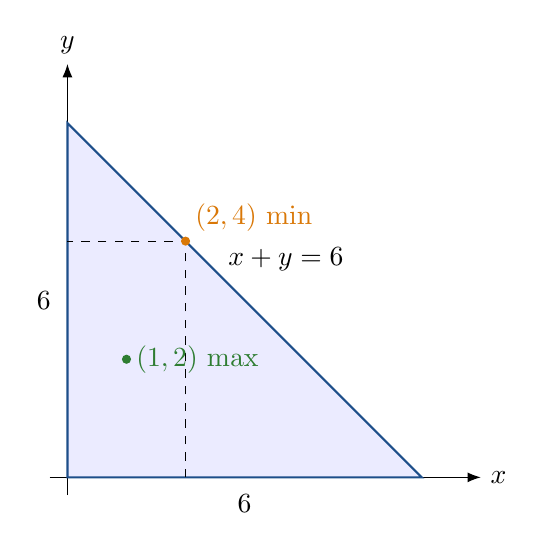
\begin{tikzpicture}[scale=0.75,>=Latex]
\draw[->] (-0.3,0)--(7,0) node[right]{$x$};
\draw[->] (0,-0.3)--(0,7) node[above]{$y$};
\fill[blue!8] (0,0)--(6,0)--(0,6)--cycle;
\draw[lineblue,thick] (0,0)--(6,0)--(0,6)--cycle;
\draw[dashed] (2,0)--(2,4)--(0,4);
\fill[linegreen] (1,2) circle (2.2pt) node[right]{$(1,2)$ max};
\fill[lineorange] (2,4) circle (2.2pt) node[above right]{$(2,4)$ min};
\node at (3,-0.45){$6$};
\node at (-0.4,3){$6$};
\node at (3.7,3.7){$x+y=6$};
\end{tikzpicture}
\caption{Triangular region for Problem 2(i).  The interior point gives the maximum and a boundary point gives the minimum.}
\end{figure}

\begin{answerbox}
\[
\boxed{\text{Absolute maximum }=4\text{ at }(1,2).}
\]
\[
\boxed{\text{Absolute minimum }=-64\text{ at }(2,4).}
\]
\end{answerbox}

\subsection{Problem 2(ii)}
Find the absolute maximum and minimum of
\[
 f(x,y)=e^{-x^2-y^2}(x^2+2y^2)
\]
on
\[
 R=\{(x,y):x^2+y^2\le1\}.
\]

Use polar coordinates:
\[
 x=r\cos\theta,
\qquad y=r\sin\theta,
\qquad 0\le r\le1.
\]
Then
\[
 x^2+y^2=r^2,
\]
and
\[
 x^2+2y^2=r^2\cos^2\theta+2r^2\sin^2\theta
=r^2(\cos^2\theta+2\sin^2\theta).
\]
Since \(\cos^2\theta=1-\sin^2\theta\),
\[
 x^2+2y^2=r^2(1+\sin^2\theta).
\]
Therefore
\[
 f=e^{-r^2}r^2(1+\sin^2\theta).
\]
For fixed \(r\), the factor \(1+\sin^2\theta\) ranges from \(1\) to \(2\).  The function is always nonnegative, so the minimum is clearly
\[
 f(0,0)=0.
\]
For the maximum, maximize
\[
 2r^2e^{-r^2}
\]
on \(0\le r\le1\).  Let \(s=r^2\).  Then \(0\le s\le1\), and
\[
 s e^{-s}
\]
has derivative
\[
 e^{-s}-se^{-s}=e^{-s}(1-s).
\]
This is nonnegative on \([0,1]\) and zero only at \(s=1\).  Therefore the maximum occurs when
\[
 r=1
\]
and
\[
 \sin^2\theta=1.
\]
Thus
\[
 (x,y)=(0,1)\quad\text{or}\quad(0,-1).
\]
The maximum value is
\[
 2e^{-1}=\frac2e.
\]

\begin{figure}[H]
\centering
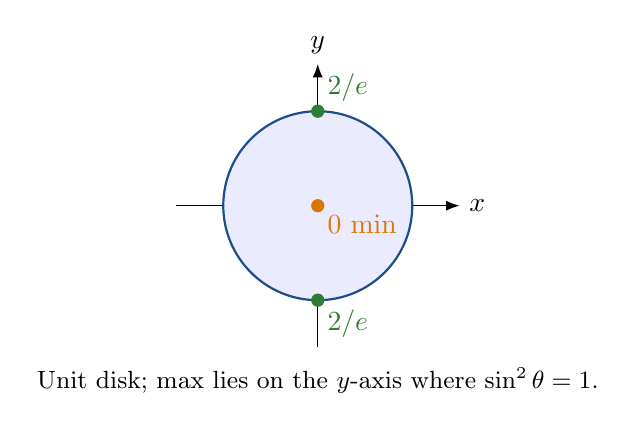
\begin{tikzpicture}[scale=1.2,>=Latex]
\draw[->] (-1.5,0)--(1.5,0) node[right]{$x$};
\draw[->] (0,-1.5)--(0,1.5) node[above]{$y$};
\fill[blue!8] (0,0) circle (1);
\draw[lineblue,thick] (0,0) circle (1);
\fill[lineorange] (0,0) circle (2pt) node[below right]{$0$ min};
\fill[linegreen] (0,1) circle (2pt) node[above right]{$2/e$};
\fill[linegreen] (0,-1) circle (2pt) node[below right]{$2/e$};
\node at (0,-1.85){\small Unit disk; max lies on the $y$-axis where $\sin^2\theta=1$.};
\end{tikzpicture}
\caption{Disk region for Problem 2(ii).}
\end{figure}

\begin{answerbox}
\[
\boxed{\text{Absolute minimum }=0\text{ at }(0,0).}
\]
\[
\boxed{\text{Absolute maximum }=\frac2e\text{ at }(0,1)\text{ and }(0,-1).}
\]
\end{answerbox}

\section{Problem 3: Double integrals as volumes}

\subsection{Problem 3(i)}
Evaluate
\[
 \iint_R 3\,dA,
\]
where
\[
 R=\{(x,y):-2\le x\le2,
\ 1\le y\le6\}.
\]

\begin{notebox}
The source scan is visually consistent with \(-2\le x\le2\).  If the lower bound were literally \(2\le x\le2\), the region would have zero width.  I use the mathematically intended rectangular region \(-2\le x\le2\).
\end{notebox}

The integrand \(3\) is a constant height above the rectangle.  The area of \(R\) is
\[
 (2-(-2))(6-1)=4\cdot5=20.
\]
Therefore the volume is
\[
 3\cdot20=60.
\]

\begin{answerbox}
\[
\boxed{\iint_R3\,dA=60.}
\]
\end{answerbox}

\subsection{Problem 3(ii)}
Evaluate
\[
 \iint_R 5x\,dA,
\]
where
\[
 R=\{(x,y):0\le x\le5,
\ 0\le y\le3\}.
\]

Write the integral explicitly:
\[
 \iint_R5x\,dA
 =\int_0^5\int_0^3 5x\,dy\,dx.
\]
First integrate with respect to \(y\):
\[
 \int_0^3 5x\,dy=5x[y]_0^3=15x.
\]
Then integrate with respect to \(x\):
\[
 \int_0^515x\,dx=15\left[\frac{x^2}{2}\right]_0^5
 =15\cdot\frac{25}{2}=\frac{375}{2}.
\]

\begin{answerbox}
\[
\boxed{\iint_R5x\,dA=\frac{375}{2}.}
\]
\end{answerbox}

\section{Problem 4: Iterated integrals}

\begin{methodbox}
For each iterated integral, I integrate from the inside outward.  Constants with respect to the current variable are pulled outside the inner integral, and every antiderivative is evaluated at both bounds.
\end{methodbox}

\subsection{Problem 4(i)}
\[
 I=\int_0^2\int_0^4 y^2e^{2x}\,dy\,dx.
\]
Since \(e^{2x}\) is constant with respect to \(y\),
\[
 \int_0^4y^2e^{2x}\,dy=e^{2x}\left[\frac{y^3}{3}\right]_0^4
 =e^{2x}\frac{64}{3}.
\]
Therefore
\[
 I=\frac{64}{3}\int_0^2e^{2x}\,dx
 =\frac{64}{3}\left[\frac12e^{2x}\right]_0^2
 =\frac{32}{3}(e^4-1).
\]
\[
\boxed{I=\frac{32}{3}(e^4-1).}
\]

\subsection{Problem 4(ii)}
\[
 I=\int_{-3}^{3}\int_0^{\pi/2}(y+y^2\cos x)\,dx\,dy.
\]
Inner integral:
\[
 \int_0^{\pi/2}(y+y^2\cos x)\,dx
 =y\left[x\right]_0^{\pi/2}+y^2\left[\sin x\right]_0^{\pi/2}
 =\frac{\pi y}{2}+y^2.
\]
Thus
\[
 I=\int_{-3}^{3}\left(\frac{\pi y}{2}+y^2\right)dy.
\]
The term \(\frac{\pi y}{2}\) is odd on \([-3,3]\), so its integral is zero.  Hence
\[
 I=\int_{-3}^{3}y^2\,dy
 =\left[\frac{y^3}{3}\right]_{-3}^{3}
 =9-(-9)=18.
\]
\[
\boxed{I=18.}
\]

\subsection{Problem 4(iii)}
\[
 I=\int_1^3\int_1^5 xy\ln y\,dy\,dx.
\]
Since \(x\) is constant in the inner integral,
\[
 I=\int_1^3 x\left(\int_1^5 y\ln y\,dy\right)dx.
\]
Use integration by parts for \(\int y\ln y\,dy\).  Let
\[
 u=\ln y,
\qquad dv=y\,dy.
\]
Then
\[
 du=\frac1y\,dy,
\qquad v=\frac{y^2}{2}.
\]
So
\[
 \int y\ln y\,dy=\frac{y^2}{2}\ln y-\int\frac{y^2}{2}\cdot\frac1y\,dy
 =\frac{y^2}{2}\ln y-\int\frac y2\,dy
 =\frac{y^2}{2}\ln y-\frac{y^2}{4}.
\]
Evaluate from \(1\) to \(5\):
\[
 \int_1^5y\ln y\,dy
 =\left[\frac{y^2}{2}\ln y-\frac{y^2}{4}\right]_1^5
 =\frac{25}{2}\ln5-\frac{25}{4}+\frac14
 =\frac{25}{2}\ln5-6.
\]
Therefore
\[
 I=\left(\frac{25}{2}\ln5-6\right)\int_1^3x\,dx
 =\left(\frac{25}{2}\ln5-6\right)\left[\frac{x^2}{2}\right]_1^3.
\]
Since
\[
 \left[\frac{x^2}{2}\right]_1^3=\frac{9-1}{2}=4,
\]
we get
\[
 I=50\ln5-24.
\]
\[
\boxed{I=50\ln5-24.}
\]

\subsection{Problem 4(iv)}
\[
 I=\int_0^1\int_0^1 v(u+v^2)^4\,du\,dv.
\]
For fixed \(v\), use \(w=u+v^2\), so \(dw=du\).  Then
\[
 \int_0^1 v(u+v^2)^4\,du
 =v\left[\frac{(u+v^2)^5}{5}\right]_0^1
 =\frac v5\left((1+v^2)^5-v^{10}\right).
\]
Thus
\[
 I=\frac15\int_0^1v(1+v^2)^5\,dv-\frac15\int_0^1v^{11}\,dv.
\]
For the first integral, let \(s=1+v^2\), so \(ds=2v\,dv\).  When \(v=0\), \(s=1\).  When \(v=1\), \(s=2\).  Hence
\[
 \int_0^1v(1+v^2)^5\,dv
 =\frac12\int_1^2s^5\,ds
 =\frac12\left[\frac{s^6}{6}\right]_1^2
 =\frac{64-1}{12}=\frac{21}{4}.
\]
The second integral is
\[
 \int_0^1v^{11}\,dv=\frac1{12}.
\]
Therefore
\[
 I=\frac15\left(\frac{21}{4}-\frac1{12}\right)
 =\frac15\left(\frac{63-1}{12}\right)
 =\frac15\cdot\frac{62}{12}
 =\frac{31}{30}.
\]
\[
\boxed{I=\frac{31}{30}.}
\]

\subsection{Problem 4(v)}
\[
 I=\int_0^1\int_0^1xy\sqrt{x^2+y^2}\,dy\,dx.
\]
For fixed \(x\), compute the inner integral:
\[
 \int xy\sqrt{x^2+y^2}\,dy=x\int y\sqrt{x^2+y^2}\,dy.
\]
Let
\[
 s=x^2+y^2,
\qquad ds=2y\,dy.
\]
Then
\[
 x\int y\sqrt{x^2+y^2}\,dy
 =\frac{x}{2}\int s^{1/2}\,ds
 =\frac{x}{2}\cdot\frac{2}{3}s^{3/2}
 =\frac{x}{3}(x^2+y^2)^{3/2}.
\]
Therefore
\[
 \int_0^1xy\sqrt{x^2+y^2}\,dy
 =\frac{x}{3}\left((x^2+1)^{3/2}-x^3\right).
\]
Now integrate in \(x\):
\[
 I=\frac13\int_0^1x(x^2+1)^{3/2}\,dx-\frac13\int_0^1x^4\,dx.
\]
For the first integral, let \(s=x^2+1\), so \(ds=2x\,dx\).  Then
\[
 \int_0^1x(x^2+1)^{3/2}\,dx
 =\frac12\int_1^2s^{3/2}\,ds
 =\frac12\left[\frac{2}{5}s^{5/2}\right]_1^2
 =\frac15(2^{5/2}-1).
\]
Also,
\[
 \int_0^1x^4\,dx=\frac15.
\]
Thus
\[
 I=\frac13\left(\frac{2^{5/2}-1}{5}-\frac15\right)
 =\frac{2^{5/2}-2}{15}.
\]
\[
\boxed{I=\frac{2^{5/2}-2}{15}.}
\]

\subsection{Problem 4(vi)}
\[
 I=\int_0^2\int_0^{\pi}r\sin^2\theta\,d\theta\,dr.
\]
Separate the variables:
\[
 I=\left(\int_0^2r\,dr\right)\left(\int_0^{\pi}\sin^2\theta\,d\theta\right).
\]
The first integral is
\[
 \int_0^2r\,dr=\left[\frac{r^2}{2}\right]_0^2=2.
\]
The standard identity
\[
 \sin^2\theta=\frac{1-\cos2\theta}{2}
\]
gives
\[
 \int_0^{\pi}\sin^2\theta\,d\theta
 =\int_0^{\pi}\frac{1-\cos2\theta}{2}\,d\theta
 =\frac{\pi}{2}.
\]
Therefore
\[
 I=2\cdot\frac{\pi}{2}=\pi.
\]
\[
\boxed{I=\pi.}
\]

\subsection{Problem 4(vii)}
\[
 I=\int_0^1\int_0^1\sqrt{s+t}\,ds\,dt.
\]
For fixed \(t\),
\[
 \int\sqrt{s+t}\,ds=\frac23(s+t)^{3/2}.
\]
Hence
\[
 \int_0^1\sqrt{s+t}\,ds
 =\frac23\left((1+t)^{3/2}-t^{3/2}\right).
\]
Therefore
\[
 I=\frac23\int_0^1(1+t)^{3/2}\,dt-\frac23\int_0^1t^{3/2}\,dt.
\]
Now
\[
 \int_0^1(1+t)^{3/2}\,dt=\left[\frac25(1+t)^{5/2}\right]_0^1=\frac25(2^{5/2}-1),
\]
and
\[
 \int_0^1t^{3/2}\,dt=\frac25.
\]
Thus
\[
 I=\frac23\left(\frac25(2^{5/2}-1)-\frac25\right)
 =\frac{4}{15}(2^{5/2}-2).
\]
\[
\boxed{I=\frac{4}{15}(2^{5/2}-2).}
\]

\subsection{Problem 4(viii)}
\[
 I=\int_1^2\int_0^{2z}\int_0^{\ln x}xe^y\,dy\,dx\,dz.
\]
\begin{notebox}
The inner upper bound \(\ln x\) is undefined at \(x=0\).  The integral is interpreted as an improper integral at \(x=0^+\).  After evaluating the inner integral, the resulting expression is integrable on \([0,2z]\).
\end{notebox}
Inner integral:
\[
 \int_0^{\ln x}xe^y\,dy=x[e^y]_0^{\ln x}=x(x-1)=x^2-x.
\]
Then
\[
 \int_0^{2z}(x^2-x)\,dx
 =\left[\frac{x^3}{3}-\frac{x^2}{2}\right]_0^{2z}
 =\frac{8z^3}{3}-2z^2.
\]
Finally,
\[
 I=\int_1^2\left(\frac{8z^3}{3}-2z^2\right)dz
 =\frac83\left[\frac{z^4}{4}\right]_1^2-2\left[\frac{z^3}{3}\right]_1^2.
\]
So
\[
 I=\frac23(16-1)-\frac23(8-1)
 =10-\frac{14}{3}
 =\frac{16}{3}.
\]
\[
\boxed{I=\frac{16}{3}.}
\]

\subsection{Problem 4(ix)}
\[
 I=\int_0^{\pi/2}\int_0^y\int_0^x\cos(x+y+z)\,dz\,dx\,dy.
\]
Inner integral:
\[
 \int_0^x\cos(x+y+z)\,dz
 =\left[\sin(x+y+z)\right]_0^x
 =\sin(2x+y)-\sin(x+y).
\]
Now integrate in \(x\):
\[
 \int_0^y\sin(2x+y)\,dx
 =\left[-\frac12\cos(2x+y)\right]_0^y
 =-\frac12\cos3y+\frac12\cos y.
\]
Also,
\[
 \int_0^y\sin(x+y)\,dx
 =[-\cos(x+y)]_0^y
 =-\cos2y+\cos y.
\]
Therefore the integral in \(x\) equals
\[
 -\frac12\cos3y+\frac12\cos y-(-\cos2y+\cos y)
 =-\frac12\cos3y+\cos2y-\frac12\cos y.
\]
Finally,
\[
 I=\int_0^{\pi/2}\left(-\frac12\cos3y+\cos2y-\frac12\cos y\right)dy.
\]
Thus
\[
 I=\left[-\frac16\sin3y+\frac12\sin2y-\frac12\sin y\right]_0^{\pi/2}.
\]
Evaluate at \(y=\pi/2\):
\[
 -\frac16\sin\frac{3\pi}{2}+\frac12\sin\pi-\frac12\sin\frac{\pi}{2}
 =-\frac16(-1)+0-\frac12
 =\frac16-\frac12=-\frac13.
\]
At \(y=0\), the value is \(0\).  Hence
\[
\boxed{I=-\frac13.}
\]

\subsection{Problem 4(x)}
\[
 I=\int_0^{\sqrt\pi}\int_0^x\int_0^{xz}x^2\sin y\,dy\,dz\,dx.
\]
Inner integral:
\[
 \int_0^{xz}x^2\sin y\,dy
 =x^2[-\cos y]_0^{xz}
 =x^2(1-\cos(xz)).
\]
Then
\[
 \int_0^x x^2(1-\cos(xz))\,dz
 =x^2\left[z-\frac{\sin(xz)}{x}\right]_0^x
 =x^3-x\sin(x^2).
\]
Therefore
\[
 I=\int_0^{\sqrt\pi}(x^3-x\sin(x^2))\,dx.
\]
The first integral is
\[
 \int_0^{\sqrt\pi}x^3\,dx=\left[\frac{x^4}{4}\right]_0^{\sqrt\pi}=\frac{\pi^2}{4}.
\]
For the second integral, let \(u=x^2\), so \(du=2x\,dx\). Then
\[
 \int_0^{\sqrt\pi}x\sin(x^2)\,dx=\frac12\int_0^{\pi}\sin u\,du
 =\frac12[-\cos u]_0^{\pi}=\frac12(2)=1.
\]
Thus
\[
\boxed{I=\frac{\pi^2}{4}-1.}
\]

\section{Problem 5: Double integrals over specified regions}

\subsection{Problem 5(i)}
Compute
\[
 \iint_R\sin(x-y)\,dA,
\qquad R=\left\{(x,y):0\le x\le\frac\pi2,
\ 0\le y\le\frac\pi2\right\}.
\]

\[
 I=\int_0^{\pi/2}\int_0^{\pi/2}\sin(x-y)\,dy\,dx.
\]
Since
\[
 \frac{d}{dy}\cos(x-y)=\sin(x-y),
\]
we get
\[
 \int_0^{\pi/2}\sin(x-y)\,dy
 =\left[\cos(x-y)\right]_0^{\pi/2}
 =\cos\left(x-\frac\pi2\right)-\cos x.
\]
Because \(\cos(x-\pi/2)=\sin x\),
\[
 I=\int_0^{\pi/2}(\sin x-\cos x)\,dx
 =[-\cos x-\sin x]_0^{\pi/2}=0.
\]
\[
\boxed{I=0.}
\]

\subsection{Problem 5(ii)}
Compute
\[
 \iint_R\left(y+xy^{-2}\right)dA,
\qquad R=\{(x,y):0\le x\le2,
\ 1\le y\le2\}.
\]
\[
 I=\int_0^2\int_1^2\left(y+xy^{-2}\right)dy\,dx.
\]
Inner integral:
\[
 \int_1^2y\,dy=\frac{3}{2},
\qquad
 \int_1^2xy^{-2}\,dy=x[-y^{-1}]_1^2=x\left(-\frac12+1\right)=\frac{x}{2}.
\]
Thus
\[
 I=\int_0^2\left(\frac32+\frac x2\right)dx
 =\left[\frac{3x}{2}+\frac{x^2}{4}\right]_0^2
 =3+1=4.
\]
\[
\boxed{I=4.}
\]

\subsection{Problem 5(iii)}
Compute
\[
 \iint_R(x^2+2y)dA,
\]
where \(R\) is bounded by \(y=0\), \(y=x^2\), and \(x=1\).

The region is
\[
 0\le x\le1,
\qquad 0\le y\le x^2.
\]
Therefore
\[
 I=\int_0^1\int_0^{x^2}(x^2+2y)dy\,dx.
\]
Inner integral:
\[
 \int_0^{x^2}(x^2+2y)dy
 =\left[x^2y+y^2\right]_0^{x^2}
 =x^4+x^4=2x^4.
\]
Thus
\[
 I=\int_0^12x^4\,dx=2\left[\frac{x^5}{5}\right]_0^1=\frac25.
\]

\begin{figure}[H]
\centering
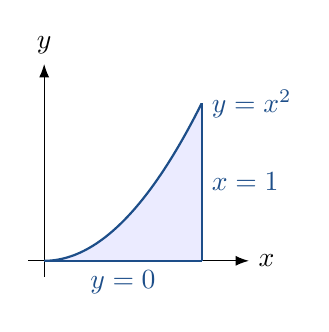
\begin{tikzpicture}[scale=2.0,>=Latex]
\draw[->] (-0.1,0)--(1.3,0) node[right]{$x$};
\draw[->] (0,-0.1)--(0,1.25) node[above]{$y$};
\fill[blue!8,domain=0:1,samples=60] (0,0)--plot({\x},{\x*\x})--(1,0)--cycle;
\draw[lineblue,thick,domain=0:1,samples=60] plot({\x},{\x*\x}) node[right]{$y=x^2$};
\draw[lineblue,thick] (0,0)--(1,0) node[midway,below]{$y=0$};
\draw[lineblue,thick] (1,0)--(1,1) node[midway,right]{$x=1$};
\end{tikzpicture}
\caption{Region for Problem 5(iii).}
\end{figure}

\[
\boxed{I=\frac25.}
\]

\subsection{Problem 5(iv)}
Compute
\[
 \iint_R y^2\,dA,
\]
where \(R\) is the triangle with vertices \((0,1),(1,2),(4,1)\).

Use horizontal slices.  The left edge from \((0,1)\) to \((1,2)\) is
\[
 y=x+1
\quad\Longrightarrow\quad
x=y-1.
\]
The right edge from \((1,2)\) to \((4,1)\) has slope
\[
 \frac{1-2}{4-1}=-\frac13.
\]
Using point \((1,2)\),
\[
 y-2=-\frac13(x-1)
\quad\Longrightarrow\quad
x=7-3y.
\]
The vertical range is \(1\le y\le2\).  Hence
\[
 I=\int_1^2\int_{y-1}^{7-3y}y^2\,dx\,dy.
\]
Inner integral:
\[
 \int_{y-1}^{7-3y}y^2\,dx=y^2\left[(7-3y)-(y-1)\right]
 =y^2(8-4y).
\]
Therefore
\[
 I=\int_1^2(8y^2-4y^3)dy
 =\left[\frac{8y^3}{3}-y^4\right]_1^2.
\]
At \(y=2\), this is
\[
 \frac{64}{3}-16=\frac{16}{3}.
\]
At \(y=1\), this is
\[
 \frac{8}{3}-1=\frac{5}{3}.
\]
Thus
\[
 I=\frac{16}{3}-\frac{5}{3}=\frac{11}{3}.
\]

\begin{figure}[H]
\centering
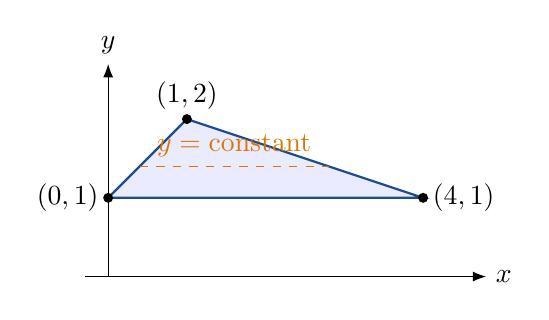
\begin{tikzpicture}[scale=1.0,>=Latex]
\draw[->] (-0.3,0)--(4.8,0) node[right]{$x$};
\draw[->] (0,0)--(0,2.7) node[above]{$y$};
\fill[blue!8] (0,1)--(1,2)--(4,1)--cycle;
\draw[lineblue,thick] (0,1)--(1,2)--(4,1)--cycle;
\fill (0,1) circle (1.8pt) node[left]{$(0,1)$};
\fill (1,2) circle (1.8pt) node[above]{$(1,2)$};
\fill (4,1) circle (1.8pt) node[right]{$(4,1)$};
\draw[dashed,lineorange] (0.4,1.4)--(2.8,1.4) node[midway,above]{$y=\text{constant}$};
\end{tikzpicture}
\caption{Horizontal slicing for Problem 5(iv).}
\end{figure}

\[
\boxed{I=\frac{11}{3}.}
\]

\subsection{Problem 5(v)}
Compute
\[
 \iint_R xy^2\,dA,
\]
where \(R\) is enclosed by
\[
 x=0
\quad\text{and}\quad
x=\sqrt{1-y^2}.
\]
This is the right half of the unit disk:
\[
 -1\le y\le1,
\qquad 0\le x\le\sqrt{1-y^2}.
\]
Thus
\[
 I=\int_{-1}^{1}\int_0^{\sqrt{1-y^2}}xy^2\,dx\,dy.
\]
Inner integral:
\[
 \int_0^{\sqrt{1-y^2}}xy^2\,dx
 =y^2\left[\frac{x^2}{2}\right]_0^{\sqrt{1-y^2}}
 =\frac12y^2(1-y^2).
\]
So
\[
 I=\frac12\int_{-1}^{1}(y^2-y^4)dy.
\]
Since the integrand is even,
\[
 I=\int_0^1(y^2-y^4)dy
 =\left[\frac{y^3}{3}-\frac{y^5}{5}\right]_0^1
 =\frac13-\frac15=\frac{2}{15}.
\]
\[
\boxed{I=\frac{2}{15}.}
\]

\subsection{Problem 5(vi)}
Compute
\[
 \iint_R\sin(x^2+y^2)dA,
\]
where \(R\) is the first-quadrant region between
\[
 x^2+y^2=a^2
\quad\text{and}\quad
x^2+y^2=b^2,
\qquad 0<a<b.
\]
Use polar coordinates.  The region is
\[
 a\le r\le b,
\qquad 0\le\theta\le\frac\pi2.
\]
Also,
\[
 x^2+y^2=r^2,
\qquad dA=r\,dr\,d\theta.
\]
So
\[
 I=\int_0^{\pi/2}\int_a^b\sin(r^2)r\,dr\,d\theta.
\]
Let \(u=r^2\), so \(du=2r\,dr\). Then
\[
 \int_a^b\sin(r^2)r\,dr
 =\frac12\int_{a^2}^{b^2}\sin u\,du
 =\frac12[-\cos u]_{a^2}^{b^2}
 =\frac12(\cos a^2-\cos b^2).
\]
Therefore
\[
 I=\frac\pi2\cdot\frac12(\cos a^2-\cos b^2)
 =\frac\pi4(\cos a^2-\cos b^2).
\]
\[
\boxed{I=\frac\pi4(\cos a^2-\cos b^2).}
\]

\subsection{Problem 5(vii)}
Compute
\[
 \iint_R e^{-x^2-y^2}dA,
\]
where \(R\) is bounded by the semicircle
\[
 x=\sqrt{4-y^2}
\]
and the \(y\)-axis.

This is the right half-disk of radius \(2\):
\[
 0\le r\le2,
\qquad -\frac\pi2\le\theta\le\frac\pi2.
\]
Thus
\[
 I=\int_{-\pi/2}^{\pi/2}\int_0^2e^{-r^2}r\,dr\,d\theta.
\]
Let \(u=r^2\), so \(du=2r\,dr\). Then
\[
 \int_0^2e^{-r^2}r\,dr
 =\frac12\int_0^4e^{-u}\,du
 =\frac12[-e^{-u}]_0^4
 =\frac12(1-e^{-4}).
\]
The angular length is \(\pi\), so
\[
 I=\pi\cdot\frac12(1-e^{-4})
 =\frac\pi2(1-e^{-4}).
\]
\[
\boxed{I=\frac\pi2(1-e^{-4}).}
\]

\subsection{Problem 5(viii)}
Compute
\[
 \iint_R\arctan\frac{y}{x}\,dA,
\]
where
\[
 R=\{(x,y):1\le x^2+y^2\le4,
\ 0\le y\le x\}.
\]
Use polar coordinates.  Since
\[
 \arctan\frac{y}{x}=\theta
\]
in the first quadrant, and the condition \(0\le y\le x\) gives
\[
 0\le\theta\le\frac\pi4.
\]
The annulus condition gives
\[
 1\le r\le2.
\]
Thus
\[
 I=\int_0^{\pi/4}\int_1^2 \theta r\,dr\,d\theta.
\]
Inner integral:
\[
 \int_1^2\theta r\,dr=\theta\left[\frac{r^2}{2}\right]_1^2=\frac32\theta.
\]
Therefore
\[
 I=\frac32\int_0^{\pi/4}\theta\,d\theta
 =\frac32\left[\frac{\theta^2}{2}\right]_0^{\pi/4}
 =\frac34\cdot\frac{\pi^2}{16}
 =\frac{3\pi^2}{64}.
\]
\[
\boxed{I=\frac{3\pi^2}{64}.}
\]

\begin{figure}[H]
\centering
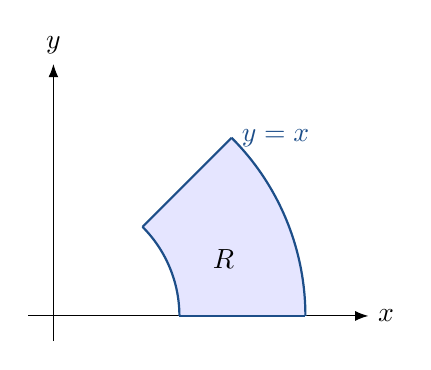
\begin{tikzpicture}[scale=1.6,>=Latex]
\draw[->] (-0.2,0)--(2.5,0) node[right]{$x$};
\draw[->] (0,-0.2)--(0,2.0) node[above]{$y$};
\fill[blue!10] (1,0) arc (0:45:1)--(1.414,1.414) arc (45:0:2)--cycle;
\draw[lineblue,thick] (1,0) arc (0:45:1);
\draw[lineblue,thick] (2,0) arc (0:45:2);
\draw[lineblue,thick] (1,0)--(2,0);
\draw[lineblue,thick] (0.707,0.707)--(1.414,1.414) node[right]{$y=x$};
\node at (1.35,0.45){$R$};
\end{tikzpicture}
\caption{Polar annular sector for Problem 5(viii).}
\end{figure}

\section{Problem 6: Volumes of solids}

\subsection{Problem 6(i)}
Find the volume bounded by
\[
 z=1-x^2-y^2
\]
and the \(xy\)-plane.

Use polar coordinates.  The \(xy\)-plane is \(z=0\), so the top surface must satisfy
\[
 1-r^2\ge0
\quad\Longrightarrow\quad
0\le r\le1.
\]
Thus
\[
 V=\int_0^{2\pi}\int_0^1(1-r^2)r\,dr\,d\theta.
\]
Compute:
\[
 \int_0^1(1-r^2)r\,dr=\int_0^1(r-r^3)dr
 =\left[\frac{r^2}{2}-\frac{r^4}{4}\right]_0^1
 =\frac12-\frac14=\frac14.
\]
Therefore
\[
 V=2\pi\cdot\frac14=\frac\pi2.
\]
\[
\boxed{V=\frac\pi2.}
\]

\subsection{Problem 6(ii)}
Find the volume under the cone
\[
 z=\sqrt{x^2+y^2}
\]
and above the disk
\[
 x^2+y^2\le4.
\]
In polar coordinates, \(z=r\) and \(0\le r\le2\).  Therefore
\[
 V=\int_0^{2\pi}\int_0^2 r\cdot r\,dr\,d\theta
 =\int_0^{2\pi}\int_0^2r^2\,dr\,d\theta.
\]
So
\[
 V=2\pi\left[\frac{r^3}{3}\right]_0^2
 =2\pi\cdot\frac83
 =\frac{16\pi}{3}.
\]
\[
\boxed{V=\frac{16\pi}{3}.}
\]

\subsection{Problem 6(iii)}
Find the volume below
\[
 z=18-2x^2-2y^2
\]
and above the \(xy\)-plane.

In polar coordinates,
\[
 z=18-2r^2.
\]
The solid exists where
\[
 18-2r^2\ge0
\quad\Longrightarrow\quad
r^2\le9
\quad\Longrightarrow\quad
0\le r\le3.
\]
Therefore
\[
 V=\int_0^{2\pi}\int_0^3(18-2r^2)r\,dr\,d\theta.
\]
Compute the radial integral:
\[
 \int_0^3(18r-2r^3)dr
 =\left[9r^2-\frac{r^4}{2}\right]_0^3
 =81-\frac{81}{2}=\frac{81}{2}.
\]
Thus
\[
 V=2\pi\cdot\frac{81}{2}=81\pi.
\]
\[
\boxed{V=81\pi.}
\]

\subsection{Problem 6(iv)}
Find the volume enclosed by the hyperboloid
\[
 -x^2-y^2+z^2=1
\]
and the plane
\[
 z=2.
\]
Rewrite the hyperboloid in cylindrical coordinates:
\[
 z^2-r^2=1.
\]
The upper sheet is
\[
 z=\sqrt{1+r^2}.
\]
The plane \(z=2\) intersects it when
\[
 2=\sqrt{1+r^2}
\quad\Longrightarrow\quad
4=1+r^2
\quad\Longrightarrow\quad
r=\sqrt3.
\]
Therefore
\[
 V=\int_0^{2\pi}\int_0^{\sqrt3}\left(2-\sqrt{1+r^2}\right)r\,dr\,d\theta.
\]
Radial integral:
\[
 \int_0^{\sqrt3}2r\,dr=3.
\]
For the second part, let \(u=1+r^2\), so \(du=2r\,dr\):
\[
 \int_0^{\sqrt3}r\sqrt{1+r^2}\,dr
 =\frac12\int_1^4u^{1/2}\,du
 =\frac12\left[\frac23u^{3/2}\right]_1^4
 =\frac13(8-1)=\frac73.
\]
Thus the radial integral is
\[
 3-\frac73=\frac23.
\]
Hence
\[
 V=2\pi\cdot\frac23=\frac{4\pi}{3}.
\]
\[
\boxed{V=\frac{4\pi}{3}.}
\]

\subsection{Problem 6(v)}
Find the volume inside the sphere
\[
 x^2+y^2+z^2=16
\]
and outside the cylinder
\[
 x^2+y^2=4.
\]
In cylindrical coordinates, the sphere is
\[
 r^2+z^2=16,
\]
so
\[
 -\sqrt{16-r^2}\le z\le\sqrt{16-r^2}.
\]
Outside the cylinder \(r=2\) and inside the sphere gives
\[
 2\le r\le4.
\]
Thus
\[
 V=\int_0^{2\pi}\int_2^4\int_{-\sqrt{16-r^2}}^{\sqrt{16-r^2}}r\,dz\,dr\,d\theta.
\]
Inner integral:
\[
 \int_{-\sqrt{16-r^2}}^{\sqrt{16-r^2}}r\,dz
 =2r\sqrt{16-r^2}.
\]
Therefore
\[
 V=\int_0^{2\pi}\int_2^4 2r\sqrt{16-r^2}\,dr\,d\theta.
\]
Let \(u=16-r^2\), so \(du=-2r\,dr\).  Then
\[
 \int_2^4 2r\sqrt{16-r^2}\,dr
 =-\int_{12}^{0}u^{1/2}\,du
 =\int_0^{12}u^{1/2}\,du
 =\left[\frac23u^{3/2}\right]_0^{12}.
\]
Now
\[
 12^{3/2}=12\sqrt{12}=24\sqrt3.
\]
So the radial part is
\[
 \frac23\cdot24\sqrt3=16\sqrt3.
\]
Finally,
\[
 V=2\pi\cdot16\sqrt3=32\pi\sqrt3.
\]
\[
\boxed{V=32\pi\sqrt3.}
\]

\begin{figure}[H]
\centering
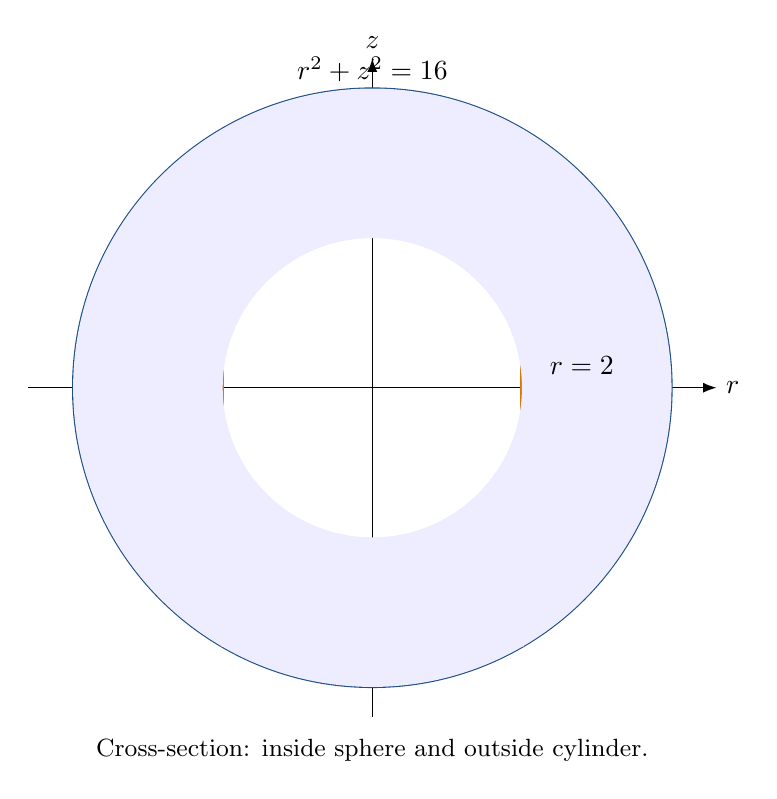
\begin{tikzpicture}[scale=0.95,>=Latex]
\draw[->] (-4.6,0)--(4.6,0) node[right]{$r$};
\draw[->] (0,-4.4)--(0,4.4) node[above]{$z$};
\draw[lineblue,thick] (0,0) circle (4);
\draw[lineorange,very thick] (2,-3.464)--(2,3.464);
\draw[lineorange,very thick] (-2,-3.464)--(-2,3.464);
\fill[blue!7,even odd rule] (0,0) circle (4) (0,0) circle (2);
\node at (0,4.25){$r^2+z^2=16$};
\node at (2.8,0.3){$r=2$};
\node at (0,-4.85){\small Cross-section: inside sphere and outside cylinder.};
\end{tikzpicture}
\caption{Meridian cross-section for Problem 6(v).}
\end{figure}

\section{Problem 7: Triple integrals over specified solids}

\subsection{Problem 7(i)}
Compute
\[
 \iiint_V y\,dV,
\]
where
\[
 V=\{(x,y,z):0\le x\le3,
\ 0\le y\le x,
\ x-y\le z\le x+y\}.
\]
Write the integral:
\[
 I=\int_0^3\int_0^x\int_{x-y}^{x+y}y\,dz\,dy\,dx.
\]
Inner integral:
\[
 \int_{x-y}^{x+y}y\,dz=y[(x+y)-(x-y)]=2y^2.
\]
Thus
\[
 I=\int_0^3\int_0^x2y^2\,dy\,dx
 =\int_0^3\left[\frac{2y^3}{3}\right]_0^x dx
 =\int_0^3\frac{2x^3}{3}dx.
\]
So
\[
 I=\frac23\left[\frac{x^4}{4}\right]_0^3
 =\frac23\cdot\frac{81}{4}
 =\frac{27}{2}.
\]
\[
\boxed{I=\frac{27}{2}.}
\]

\subsection{Problem 7(ii)}
Compute
\[
 \iiint_V \frac{z}{x^2+y^2}\,dV,
\]
where
\[
 V=\{(x,y,z):1\le y\le4,
\ y\le z\le4,
\ 0\le x\le z\}.
\]

The integral is
\[
 I=\int_1^4\int_y^4\int_0^z\frac{z}{x^2+y^2}\,dx\,dz\,dy.
\]
Integrate first with respect to \(x\):
\[
 \int_0^z\frac{z}{x^2+y^2}\,dx
 =z\left[\frac1y\arctan\frac{x}{y}\right]_0^z
 =\frac{z}{y}\arctan\frac{z}{y}.
\]
Thus an exact reduced form is
\[
 I=\int_1^4\int_y^4\frac{z}{y}\arctan\frac{z}{y}\,dz\,dy.
\]
This double integral can also be reduced by changing order after integrating in \(z\).  Since
\[
 1\le y\le4,
\qquad y\le z\le4,
\qquad 0\le x\le z,
\]
we can integrate \(z\) first for fixed \((x,y)\).  Then
\[
 z\in[\max(x,y),4].
\]
Splitting into \(0\le x\le y\) and \(y\le x\le4\), we get
\[
 I=\int_1^4\left[\int_0^y\frac{16-y^2}{2(x^2+y^2)}\,dx
 +\int_y^4\frac{16-x^2}{2(x^2+y^2)}\,dx\right]dy.
\]
The first part is elementary:
\[
 \int_1^4\int_0^y\frac{16-y^2}{2(x^2+y^2)}\,dx\,dy
 =\frac\pi8\int_1^4\left(\frac{16}{y}-y\right)dy
 =\frac\pi8\left(16\ln4-\frac{15}{2}\right).
\]
The second part is left in a one-dimensional exact integral form:
\[
 \frac12\int_1^4\left(\frac{16}{x}-x\right)\left(\frac\pi4-\arctan\frac1x\right)dx.
\]
Therefore
\[
 I=\frac\pi8\left(16\ln4-\frac{15}{2}\right)
 +\frac12\int_1^4\left(\frac{16}{x}-x\right)\left(\frac\pi4-\arctan\frac1x\right)dx.
\]
A numerical evaluation gives
\[
 I\approx 7.587351988.
\]

\begin{answerbox}
\[
\boxed{I=\frac\pi8\left(16\ln4-\frac{15}{2}\right)
 +\frac12\int_1^4\left(\frac{16}{x}-x\right)\left(\frac\pi4-\arctan\frac1x\right)dx
 \approx7.587351988.}
\]
\end{answerbox}

\subsection{Problem 7(iii)}
Compute
\[
 \iiint_V\sin y\,dV,
\]
where \(V\) is below the plane \(z=x\) and above the triangular region with vertices
\[
 (0,0,0),\quad(\pi,0,0),\quad(0,\pi,0).
\]
The base region in the \(xy\)-plane is
\[
 x\ge0,
\qquad y\ge0,
\qquad x+y\le\pi.
\]
The height is
\[
 0\le z\le x.
\]
Therefore
\[
 I=\int_0^\pi\int_0^{\pi-y}\int_0^x\sin y\,dz\,dx\,dy.
\]
Inner integral:
\[
 \int_0^x\sin y\,dz=x\sin y.
\]
Then
\[
 I=\int_0^\pi\int_0^{\pi-y}x\sin y\,dx\,dy
 =\int_0^\pi\sin y\left[\frac{x^2}{2}\right]_0^{\pi-y}dy.
\]
Thus
\[
 I=\frac12\int_0^\pi(\pi-y)^2\sin y\,dy.
\]
Let \(u=\pi-y\).  Then \(dy=-du\), and \(\sin y=\sin(\pi-u)=\sin u\).  The bounds change from \(y=0\) to \(u=\pi\), and from \(y=\pi\) to \(u=0\).  Therefore
\[
 I=\frac12\int_0^\pi u^2\sin u\,du.
\]
Integrating by parts twice gives
\[
 \int_0^\pi u^2\sin u\,du=\pi^2-4.
\]
Therefore
\[
\boxed{I=\frac{\pi^2-4}{2}.}
\]

\subsection{Problem 7(iv)}
Compute
\[
 \iiint_Vxy\,dV,
\]
where \(V\) is bounded by the parabolic cylinders
\[
 y=x^2,
\qquad x=y^2,
\]
and the planes
\[
 z=0,
\qquad z=x+y.
\]
The two parabolas meet at \((0,0)\) and \((1,1)\).  In the first quadrant, the base region is
\[
 0\le x\le1,
\qquad x^2\le y\le\sqrt{x}.
\]
The height is
\[
 0\le z\le x+y.
\]
Thus
\[
 I=\int_0^1\int_{x^2}^{\sqrt{x}}\int_0^{x+y}xy\,dz\,dy\,dx.
\]
Inner integral:
\[
 \int_0^{x+y}xy\,dz=xy(x+y).
\]
Therefore
\[
 I=\int_0^1\int_{x^2}^{\sqrt{x}}(x^2y+xy^2)\,dy\,dx.
\]
Compute the inner integral:
\[
 \int(x^2y+xy^2)dy=\frac{x^2y^2}{2}+\frac{xy^3}{3}.
\]
Evaluate from \(y=x^2\) to \(y=\sqrt{x}\):
\[
 \left(\frac{x^2\cdot x}{2}+\frac{x\cdot x^{3/2}}{3}\right)
 -\left(\frac{x^2\cdot x^4}{2}+\frac{x\cdot x^6}{3}\right)
 =\frac{x^3}{2}+\frac{x^{5/2}}{3}-\frac{x^6}{2}-\frac{x^7}{3}.
\]
Now integrate from \(0\) to \(1\):
\[
 I=\int_0^1\left(\frac{x^3}{2}+\frac{x^{5/2}}{3}-\frac{x^6}{2}-\frac{x^7}{3}\right)dx.
\]
Thus
\[
 I=\frac12\cdot\frac14+\frac13\cdot\frac{2}{7}-\frac12\cdot\frac17-\frac13\cdot\frac18.
\]
Compute the fractions:
\[
 I=\frac18+\frac{2}{21}-\frac1{14}-\frac1{24}=\frac{3}{28}.
\]
\[
\boxed{I=\frac{3}{28}.}
\]

\subsection{Problem 7(v)}
Compute
\[
 \iiint_Vx^2\,dV,
\]
where \(V\) is the tetrahedron with vertices
\[
 (0,0,0),\quad(1,0,0),\quad(0,1,0),\quad(0,0,1).
\]
The tetrahedron is
\[
 x\ge0,
\qquad y\ge0,
\qquad z\ge0,
\qquad x+y+z\le1.
\]
Thus
\[
 0\le x\le1,
\qquad 0\le y\le1-x,
\qquad 0\le z\le1-x-y.
\]
So
\[
 I=\int_0^1\int_0^{1-x}\int_0^{1-x-y}x^2\,dz\,dy\,dx.
\]
Inner integral:
\[
 \int_0^{1-x-y}x^2\,dz=x^2(1-x-y).
\]
Then
\[
 \int_0^{1-x}x^2(1-x-y)dy
 =x^2\left[(1-x)y-\frac{y^2}{2}\right]_0^{1-x}
 =x^2\cdot\frac{(1-x)^2}{2}.
\]
Therefore
\[
 I=\frac12\int_0^1x^2(1-x)^2dx.
\]
Expand:
\[
 x^2(1-x)^2=x^2-2x^3+x^4.
\]
Hence
\[
 I=\frac12\left(\frac13-\frac12+\frac15\right)
 =\frac12\cdot\frac1{30}
 =\frac1{60}.
\]
\[
\boxed{I=\frac1{60}.}
\]

\section{Problem 8: Change the order of integration}

\subsection{Problem 8(i)}
Given
\[
 \int_0^1\left[\int_0^y f(x,y)\,dx\right]dy.
\]
The region is
\[
 0\le y\le1,
\qquad 0\le x\le y.
\]
This means
\[
 0\le x\le y\le1.
\]
If we describe it with \(x\) first, then
\[
 0\le x\le1,
\qquad x\le y\le1.
\]
Therefore
\[
\boxed{\int_0^1\int_0^y f(x,y)\,dx\,dy
=\int_0^1\int_x^1f(x,y)\,dy\,dx.}
\]

\begin{figure}[H]
\centering
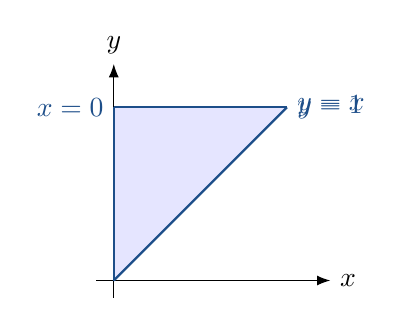
\begin{tikzpicture}[scale=2.2,>=Latex]
\draw[->] (-0.1,0)--(1.25,0) node[right]{$x$};
\draw[->] (0,-0.1)--(0,1.25) node[above]{$y$};
\fill[blue!10] (0,0)--(0,1)--(1,1)--cycle;
\draw[lineblue,thick] (0,0)--(1,1) node[right]{$y=x$};
\draw[lineblue,thick] (0,1)--(1,1) node[right]{$y=1$};
\draw[lineblue,thick] (0,0)--(0,1) node[left]{$x=0$};
\end{tikzpicture}
\caption{Region \(0\le x\le y\le1\).}
\end{figure}

\subsection{Problem 8(ii)}
Given
\[
 \int_0^2\left[\int_{2y}^{y^2} f(x,y)\,dx\right]dy.
\]
For \(0<y<2\), we have
\[
 y^2<2y.
\]
So the given integral has reversed inner bounds.  The geometric region between the curves is
\[
 y^2\le x\le2y,
\qquad 0\le y\le2.
\]
The original integral is therefore the negative of the positively oriented integral over this region:
\[
 \int_0^2\int_{2y}^{y^2}f(x,y)\,dx\,dy
 =-\int_0^2\int_{y^2}^{2y}f(x,y)\,dx\,dy.
\]
Now solve the boundary equations for \(y\):
\[
 x=y^2\quad\Longrightarrow\quad y=\sqrt{x},
\]
and
\[
 x=2y\quad\Longrightarrow\quad y=\frac{x}{2}.
\]
The curves intersect at \(y=0,2\), giving \(x=0,4\).  For \(0\le x\le4\),
\[
 \frac{x}{2}\le y\le\sqrt{x}.
\]
Thus
\[
\boxed{\int_0^2\int_{2y}^{y^2}f(x,y)\,dx\,dy
=-\int_0^4\int_{x/2}^{\sqrt{x}}f(x,y)\,dy\,dx.}
\]
Equivalently, preserving reversed orientation inside,
\[
\boxed{\int_0^2\int_{2y}^{y^2}f(x,y)\,dx\,dy
=\int_0^4\int_{\sqrt{x}}^{x/2}f(x,y)\,dy\,dx.}
\]

\begin{figure}[H]
\centering
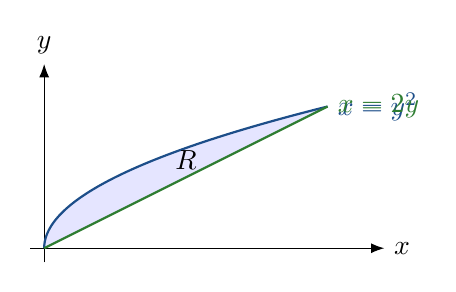
\begin{tikzpicture}[scale=0.9,>=Latex]
\draw[->] (-0.2,0)--(4.8,0) node[right]{$x$};
\draw[->] (0,-0.2)--(0,2.6) node[above]{$y$};
\fill[blue!10,domain=0:2,samples=80] plot({\x*\x},{\x})--plot[domain=2:0]({2*\x},{\x})--cycle;
\draw[lineblue,thick,domain=0:2,samples=80] plot({\x*\x},{\x}) node[right]{$x=y^2$};
\draw[linegreen,thick,domain=0:2,samples=80] plot({2*\x},{\x}) node[right]{$x=2y$};
\node at (2.0,1.25){$R$};
\end{tikzpicture}
\caption{Region between \(x=y^2\) and \(x=2y\).  The original integral uses reversed inner limits.}
\end{figure}

\subsection{Problem 8(iii)}
The printed variables are inconsistent in the scan.  The standard consistent reading is
\[
 \int_1^e\left[\int_0^{\ln x}f(x,y)\,dy\right]dx.
\]
The region is
\[
 1\le x\le e,
\qquad 0\le y\le\ln x.
\]
The inequality \(y\le\ln x\) is equivalent to
\[
 x\ge e^y.
\]
Since \(x\le e\), the maximum value of \(y\) is \(1\).  Therefore the changed order is
\[
 0\le y\le1,
\qquad e^y\le x\le e.
\]
Thus
\[
\boxed{\int_1^e\int_0^{\ln x}f(x,y)\,dy\,dx
=\int_0^1\int_{e^y}^{e}f(x,y)\,dx\,dy.}
\]

\begin{figure}[H]
\centering
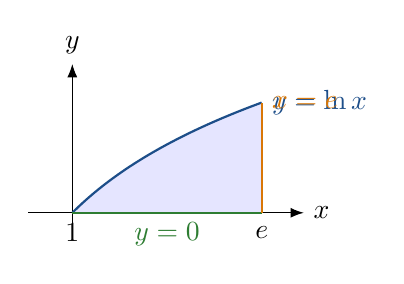
\begin{tikzpicture}[scale=1.4,>=Latex]
\draw[->] (0.6,0)--(3.1,0) node[right]{$x$};
\draw[->] (1,-0.1)--(1,1.35) node[above]{$y$};
\fill[blue!10,domain=1:2.718,samples=80] (1,0)--plot({\x},{ln(\x)})--(2.718,0)--cycle;
\draw[lineblue,thick,domain=1:2.718,samples=80] plot({\x},{ln(\x)}) node[right]{$y=\ln x$};
\draw[linegreen,thick] (1,0)--(2.718,0) node[midway,below]{$y=0$};
\draw[lineorange,thick] (2.718,0)--(2.718,1) node[right]{$x=e$};
\node at (1.0,-0.18){$1$};
\node at (2.718,-0.18){$e$};
\end{tikzpicture}
\caption{Region under \(y=\ln x\) from \(x=1\) to \(x=e\).}
\end{figure}

\section{Problem 9: Equivalent iterated integrals}

\begin{methodbox}
The safest way to write equivalent iterated integrals is to first translate the given integral into inequalities describing the solid.  Then choose a new variable order and solve those inequalities in that order.
\end{methodbox}

\subsection{Problem 9(i)}
Given
\[
 \int_0^1\int_y^1\int_0^y f(x,y,z)\,dx\,dz\,dy.
\]
The inequalities are
\[
 0\le y\le1,
\qquad y\le z\le1,
\qquad 0\le x\le y.
\]
Equivalently,
\[
 0\le x\le y\le z\le1.
\]
Three other equivalent iterated integrals are:
\[
\boxed{\int_0^1\int_x^1\int_y^1 f(x,y,z)\,dz\,dy\,dx.}
\]
\[
\boxed{\int_0^1\int_0^z\int_0^y f(x,y,z)\,dx\,dy\,dz.}
\]
\[
\boxed{\int_0^1\int_0^z\int_x^z f(x,y,z)\,dy\,dx\,dz.}
\]

\subsection{Problem 9(ii)}
Given
\[
 \int_0^1\int_0^{1-x^2}\int_0^{1-x}f(x,y,z)\,dy\,dz\,dx.
\]
The inequalities are
\[
 0\le x\le1,
\qquad 0\le z\le1-x^2,
\qquad 0\le y\le1-x.
\]
One immediate equivalent integral is obtained by switching the independent \(y\)- and \(z\)-integrations:
\[
\boxed{\int_0^1\int_0^{1-x}\int_0^{1-x^2}f(x,y,z)\,dz\,dy\,dx.}
\]

For orders with \(x\) inside, observe that for fixed \((y,z)\),
\[
 x\le1-y,
\qquad x\le\sqrt{1-z}.
\]
Thus
\[
 0\le x\le\min(1-y,\sqrt{1-z}).
\]
The curve where the two upper bounds are equal is
\[
 1-y=\sqrt{1-z}
\quad\Longleftrightarrow\quad
 z=2y-y^2.
\]
Therefore another equivalent expression is
\[
\boxed{\int_0^1\left[
\int_0^{2y-y^2}\int_0^{1-y}f(x,y,z)\,dx\,dz
+\int_{2y-y^2}^{1}\int_0^{\sqrt{1-z}}f(x,y,z)\,dx\,dz
\right]dy.}
\]
Using \(z\) as the outer variable, the switching curve becomes
\[
 y=1-\sqrt{1-z}.
\]
Thus a third equivalent expression is
\[
\boxed{\int_0^1\left[
\int_0^{1-\sqrt{1-z}}\int_0^{\sqrt{1-z}}f(x,y,z)\,dx\,dy
+\int_{1-\sqrt{1-z}}^1\int_0^{1-y}f(x,y,z)\,dx\,dy
\right]dz.}
\]

\subsection{Problem 9(iii)}
Given
\[
 \int_0^1\int_{\sqrt{x}}^1\int_0^{1-y}f(x,y,z)\,dz\,dy\,dx.
\]
The inequalities are
\[
 0\le x\le1,
\qquad \sqrt{x}\le y\le1,
\qquad 0\le z\le1-y.
\]
The condition \(\sqrt{x}\le y\) is equivalent to
\[
 x\le y^2.
\]
Thus the solid can be written as
\[
 0\le y\le1,
\qquad 0\le x\le y^2,
\qquad 0\le z\le1-y.
\]
Three other equivalent iterated integrals are:
\[
\boxed{\int_0^1\int_0^{y^2}\int_0^{1-y}f(x,y,z)\,dz\,dx\,dy.}
\]
\[
\boxed{\int_0^1\int_0^{1-z}\int_0^{y^2}f(x,y,z)\,dx\,dy\,dz.}
\]
For fixed \((x,z)\), the inequalities require
\[
 \sqrt{x}\le y\le1-z.
\]
This is possible when
\[
 0\le z\le1-\sqrt{x}.
\]
Therefore another equivalent integral is
\[
\boxed{\int_0^1\int_0^{1-\sqrt{x}}\int_{\sqrt{x}}^{1-z}f(x,y,z)\,dy\,dz\,dx.}
\]

\section*{Visual verification notes}
\addcontentsline{toc}{section}{Visual verification notes}
This TeX file was written with TikZ diagrams for the main geometric regions and solid cross-sections.  For verification, the compiled PDF should be rendered page-by-page.  The expected visual checks are: no clipped text, no overlapping display equations, readable captions, and diagrams placed close to the computations they support.

\end{document}
